\documentclass[conference]{IEEEtran}
\IEEEoverridecommandlockouts
% The preceding line is only needed to identify funding in the first footnote. If that is unneeded, please comment it out.
\usepackage{cite}
\usepackage{amsmath,amssymb,amsfonts}
\usepackage{algorithmic}
\usepackage{graphicx}
\usepackage{textcomp}
\usepackage{xcolor}
\def\BibTeX{{\rm B\kern-.05em{\sc i\kern-.025em b}\kern-.08em
    T\kern-.1667em\lower.7ex\hbox{E}\kern-.125emX}}
\begin{document}

\title{Distributed Systems - Surveillance System Project}

\author{\IEEEauthorblockN{1\textsuperscript{st} Cedric Sillaber}
\and
\IEEEauthorblockN{2\textsuperscript{nd} Alan Gallo}
\and
\IEEEauthorblockN{3\textsuperscript{rd} Frantisek Sova}
}

\maketitle

\section{Introduction}
In our surveillance system, cameras are simulated using the WiseNET dataset. The system is designed to capture video streams and process them efficiently for real-time object and facial recognition. The video data undergoes preprocessing at the edge, minimizing the workload on the cloud, reducing latency, and optimizing the overall performance of the surveillance system. The system leverages edge devices and cloud services to ensure scalability, fast response times, and effective monitoring.  

\section{System architecture}
The video files are stored in camera containers running on EC2 instances \ref{fig:architecture}. Each container parses a certain video file into images using OpenCV. These sequences are then sent to edge devices at regular intervals through HTTP, simulating a real-time video stream. Communication between components is handled through a WebSocket, which is capable of managing large payloads and scaling efficiently. Additionally, the EC2 instance houses an alarm container, completing the IoT layer of the system.

\begin{figure}[h!]
    \centering
    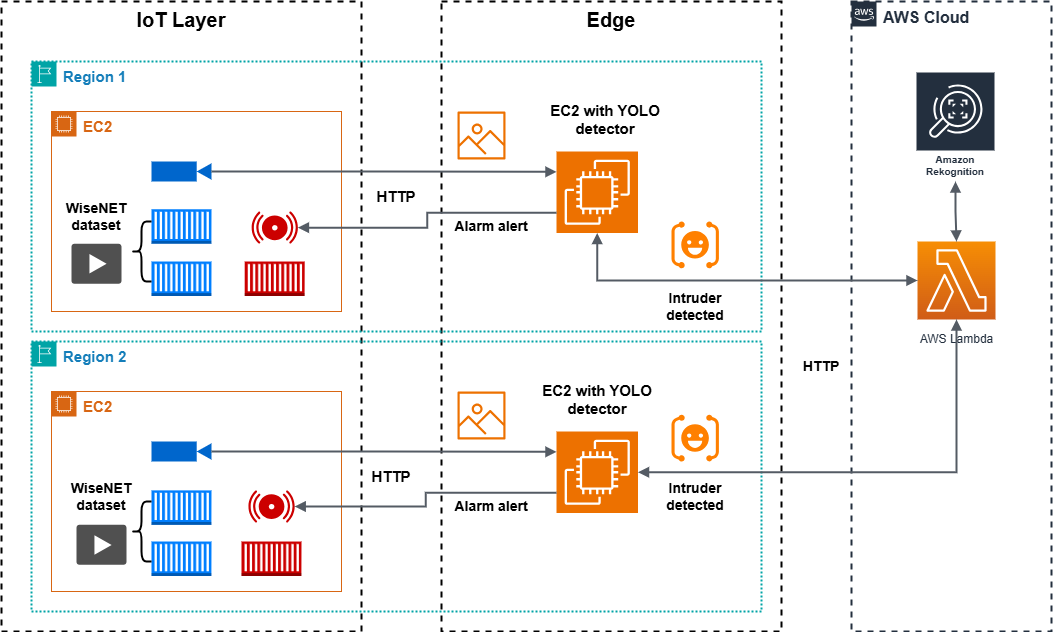
\includegraphics[width=1\linewidth]{res/report/DS_architecture_version2.png}
    \caption{Example of your architectural diagram.}
    \label{fig:architecture}
\end{figure}

The edge layer consists of two EC2 instances simulating edge devices in different locations. At the edge, the video data is processed using the YOLO (You Only Look Once) algorithm to detect objects and people. When a person-like object is detected, the relevant data is forwarded to AWS Lambda in the cloud, ensuring the system can scale dynamically based on demand.

The cloud layer integrates with Amazon Rekognition to perform facial recognition, comparing the detected face against a collection of known individuals. If an unknown person is identified, Lambda triggers an alert, which is sent back to the edge device and activates the alarm in the IoT layer. This architecture reduces the workload on the cloud, minimizes latency, and ensures the system can handle large volumes of video data in a responsive and efficient manner, making it a robust solution for surveillance applications.



\section{Implementation details}
The IoT layer is represented by 4 camera containers and one alarm container for each edge device. The simulation video comes from set\_3 of WiseNET dataset, which potrays two people appearing in differnt times on the scene. One person can simulate the intruder and the other an employee. 

While all camera containers will include the whole set of videos, each will select only one based on an environment variable bound to the container. This video is then processed using OpenCV read() function, which returns the sequence of frames. Those are then sent using Socket.IO library to the edge device in an interval simulating the real frame rate. 

The alarm container also connects to the edge server and waits for an event, that will trigger it.


\section{Evaluation}
Evaluation of the response time and scalability (number of devices and traffic) to prove the correctness of your implementation. The more detailed the better. 

\end{document}
